\part*{Task 2: Identify User, Software, and System Requirements}
\addcontentsline{toc}{part}{Task 2: - Identify User, Software, and System Requirements}

The identification of user, software, and system requirements were scraped and
    analyzed from the Google Play Store, both from the app's description and its
    reviews, and from \href{https://www.grandpad.net/}{GrandPad's website}.

\section*{Analyzing GrandPad's Google Play Description and Website}
\addcontentsline{toc}{section}{Analyzing GrandPad's Google Play Description and Website}

First, analysis was conducted on the description of the GrandPad app on the
    Google Play Store and from their website.

\subsection*{User Requirements from GrandPad's Description and Website}
\addcontentsline{toc}{subsection}{User Requirements from GrandPad's Description and Website}

The following user requirements were created from analyzing GrandPad's goals and
    desired outcomes for families.
The Google Play Store description contains many needs that GrandPad claims to
    satisfy \cite{grandpad_google_play}, and the GrandPad website lists
    product details that fill gaps for its users \cite{grandpad_product_details}.

\begin{description}
    \item[\textbf{\showusernetcounter}]
        As a member of a group of family members and friends with elderly
            members, I want to be able to make a private social network for us
            to stay connected.
    \item[\textbf{\showusernetcounter}]
        As an elderly member of a group of family members and friends, I want to
            have a private network to keep us connected without the distractions
            and complexity of modern social media.
    \item[\textbf{\showusercallcounter}]
        As a member of a GrandPad family network, I want to make video and voice
            calls to intimately connect with my loved ones.
    \item[\textbf{\showuserpostcounter}]
        As a member of a GrandPad family network, I want to share photos and
            videos to stay in touch with my family members and friends.
    \item[\textbf{\showuserpostcounter}]
        As a member of a GrandPad family network, I want to comment and react to
            posts from my family and friends to stay engaged with them and their
            lives.
    \item[\textbf{\showusergamecounter}]
        As a member of a GrandPad family network, I want to play online games
            with my elderly loved one to connect with them and keep them engaged
            cognitively.
    \item[\textbf{\showusernetcounter}]
        As a caregiver for an elderly family member, I want to be able to
            remotely configure and administer their GrandPad tablet to help them
            with problems they are having with it.
\end{description}

\section*{Analyzing GrandPad's Google Play Reviews}
\addcontentsline{toc}{section}{Analyzing GrandPad's Google Play Reviews}

Next, the reviews from the GrandPad Google Play Store app were analyzed.
The following explanation of the analysis of GrandPad's reviews is a summary of
    the Jupyter Notebook in Appendix \ref{sec:reviews_processing_notebook}.

Using the
    \href{https://pypi.org/project/google-play-scraper/}{google-play-scraper}
    Python library, reviews were scraped from the Google Play Store.
Initially, 1,823 reviews were scraped, many of which were under 10 words.
This is shown in the histogram below.
\begin{figure}[H]
    \centering
    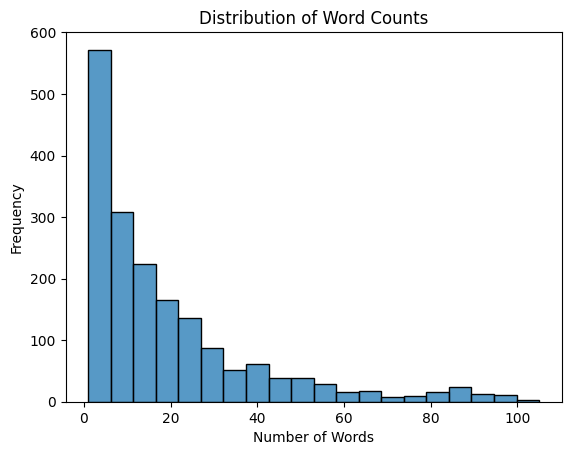
\includegraphics[width=0.75\textwidth]{images/word_length_distribution.png}
\end{figure}
To reduce the amount of data to analyze, all reviews under 10 words were
    removed.
The reviews were then split by their rating (5 stars: positive, 2-4 stars:
    mixed, 1 star: negative) and run through a
    \href
        {https://scikit-learn.org/dev/modules/generated/sklearn.decomposition.LatentDirichletAllocation.html}
        {Latent Dirichlet Allocation (LDA) algorithm from Scikit Learn}
    to identify important topics from each category of the reviews.

\subsection*{User Requirements from Negative Reviews}
\addcontentsline{toc}{subsection}{User Requirements from Negative Reviews}

The analysis of negative reviews led to some recurring topics, which included
    lack of professional support,
    intrusive app behavior,
    lack of personalization functionality,
    poor quality of video and voice calls,
    and frustrating notification experience.

\begin{description}
    \item[\textbf{\showuserhelpcounter}]
        As a member of a GrandPad family network, I need to have access to
            support staff during work hours to help configure the network.
    \item[\textbf{\showuserhelpcounter}]
        As a senior user of GrandPad, I need to have access to support staff
            during work hours to help troubleshoot problems with the GrandPad
            tablet.
    \item[\textbf{\showuseruicounter}]
        As a user of the GrandPad app, I don't want the app to override
            Do Not Disturb mode on my phone.
    \item[\textbf{\showuseruicounter}]
        As an administrator of a GrandPad network, I want to be able to
            customize the elderly user's GrandPad tablet to suit their
            proficiency and comfort levels with technology.
    \item[\textbf{\showuseruicounter}]
        As an elderly user of the GrandPad tablet who is moderately comfortable
            with technology, I want to be able to customize the my GrandPad
            tablet to add or remove features.
    \item[\textbf{\showusercallcounter}]
        As a member of a GrandPad family network, I want to video call with high
            enough quality to see and hear my loved ones.
    \item[\textbf{\showusercallcounter}]
        As a member of a GrandPad family network, I want to voice call with high
            enough quality to hear my loved ones.
    \item[\textbf{\showuserpostcounter}]
        As a user of the GrandPad app, I want to be able to receive
            notifications when a member of the network posts, comments, or
            reacts to a post, or calls me.
    \item[\textbf{\showuseruicounter}]
        As a user of the GrandPad app, I want to be able to clear all
            notifications at once, without having to individually clear each
            one.
\end{description}

\subsection*{User Requirements from Mixed Reviews}
\addcontentsline{toc}{subsection}{User Requirements from Mixed Reviews}

When analyzing the mixed reviews, some recurring topics were
    connecting multiple GrandPad tablets to a single network,
    being part of multiple networks,
    editing posts and comments,
    vague error messages,
    posting/downloading multiple files at once,
    and sending message to or calling specific people in a network.

\begin{description}
    \item[\textbf{\showusernetcounter}]
        As an administrator of a GrandPad family network, I need to be able to
            add multiple users with GrandPad tablets to a single network, to
            accommodate multiple elderly family members.
    \item[\textbf{\showusernetcounter}]
        As a user of the GrandPad app, I want to be able to easily join and
            switch between multiple GrandPad family networks because I am part
            of multiple social circles with elderly people.
    \item[\textbf{\showuserpostcounter}]
        As a user of the GrandPad app, I want to be able to edit the posts and
            comments that I make in case I wrote a typo.
    \item[\textbf{\showuseruicounter}]
        As a user of the GrandPad app, I want to know the reason when an upload
            fails so that I can take action to fix it.
    \item[\textbf{\showuserpostcounter}]
        As a user of the GrandPad app, I want to post multiple files at once
            because I have many pictures and videos from a single event that I
            want to share.
    \item[\textbf{\showuserpostcounter}]
        As a user of the GrandPad app, I want to download the files that my
            family members and friends share to have them saved on my device.
    \item[\textbf{\showusercallcounter}]
        As a caregiver of an elderly family member, I want to send messages to
            or call the elderly member specifically so that I can check up on
            them.
\end{description}

\subsection*{User Requirements from Positive Reviews}
\addcontentsline{toc}{subsection}{User Requirements from Positive Reviews}

When analyzing positive reviews, prominent topics that were found include
    positive customer service experience,
    ease of use for non-tech savvy users,
    ability to connect over geographical barriers,
    privacy,
    lack of scams and telemarketers,
    lack of advertisements,
    and ability to connect multiple generations of users.

\begin{description}
    \item[\textbf{\showuserhelpcounter}]
        As an elderly user of GrandPad, I need access to customer support that
            is patient and polite because I have difficulty using technology.
    \item[\textbf{\showuseruicounter}]
        As an elderly user of GrandPad, I need the interface to be simple enough
            to use with little to no technology experience.
    \item[\textbf{\showusernetcounter}]
        As a member of a GrandPad family network, I want to be able to stay
            connected with my loved ones even though they live far away or in
            places I cannot easily get to.
    \item[\textbf{\showusernetcounter}]
        As a member of a GrandPad family network, I don't want strangers to be
            able to join our network.
    \item[\textbf{\showusernetcounter}]
        As an administrator of a GrandPad family network, I want to be able to
            choose who can join the network to keep elderly members safe.
    \item[\textbf{\showusernetcounter}]
        As a caregiver of an elderly family member, I want the peace of mind of
            knowing that they are safe from scammers on the app.
    \item[\textbf{\showuseruicounter}]
        As a member of a GrandPad family network, I want to use the app to stay
            connected without being distracted by advertisements.
    \item[\textbf{\showuseruicounter}]
        As a younger member of a GrandPad family network, I want the app to be
            engaging for me, while being simple enough for non tech-savvy
            members to use.
\end{description}

\section*{Functional Requirements}
\addcontentsline{toc}{section}{Functional Requirements}

Many of the user requirements translate directly into functional requirements.
Going forward, ``the system'' will be used to refer to the GrandPad platform,
    including the app, tablet, and the support staff of the platform, where
    applicable.

\subsection*{Functional Requirements Related to the Creation and Administration of Private Social Networks}
\addcontentsline{toc}{subsection}{Functional Requirements Related to the Creation and Administration of Private Social Networks}

\begin{description}
    \item[\textbf{\showfuncnetcounter}]
        The system shall allow users to register for accounts with
            administrator privileges for a given social network that contains an
            elderly member.
    \item[\textbf{\showfuncnetcounter}]
        The system shall allow a user with an administrator role to create a
            private social network for their group of family members and
            friends.
    \item[\textbf{\showfuncnetcounter}]
        The system shall allow a user with an administrator role to invite
            family members and friends into their private social network.
    \item[\textbf{\showfuncnetcounter}]
        The system shall allow a user with an administrator role to view the
            people in their private social network.
    \item[\textbf{\showfuncnetcounter}]
        The system shall allow a user with an administrator role to remove
            members from their private social network.
    \item[\textbf{\showfuncnetcounter}]
        The system shall not allow any user to join a private social network
            without the approval of at least one of that network's
            administrative users.
    \item[\textbf{\showfuncnetcounter}]
        The system shall allow a user with an administrator role to remotely
            configure an elderly user's GrandPad tablet who is in the
            administrator's private social network.
\end{description}

\subsection*{Functional Requirements Related to Support Services}
\addcontentsline{toc}{subsection}{Functional Requirements Related to Support Services}

\begin{description}
    \item[\textbf{\showfunchelpcounter}]
        The system shall allow users to request to connect with a live support
            agent from the GrandPad app or GrandPad tablet.
    \item[\textbf{\showfunchelpcounter}]
        The system shall connect users requesting support with a live support
            agent during working hours (8:00 AM EST to 7:00 PM EST) within 30
            minutes.
    \item[\textbf{\showfunchelpcounter}]
        The system's support staff shall be patient with clients, understanding
            that they may have little to no experience with technology,
            achieving a greater than 90\% client satisfaction rate.
\end{description}

\subsection*{Functional Requirements Related to Video and Voice Calling}
\addcontentsline{toc}{subsection}{Functional Requirements Related to Video and Voice Calling}

\begin{description}
    \item[\textbf{\showfunccallcounter}]
        When clients have a strong network connection, the system shall allow
            users to video call with a data rate of at least 1.2Mbps supporting
            720p resolution for more than 95\% of the call duration.
        \footnote{Zoom Video Communications recommends 1.2Mbps Internet speed
            for 720p video calling \cite{zoom_system_requirements}.}
    \item[\textbf{\showfunccallcounter}]
        When clients have a weak internet connection, the system shall allow
            users to video call with a data rate of at least 600kbps for more
            than 95\% of the call duration.
        \footnote{Zoom Video Communications recommends 600kbps Internet speed
            for ``high quality video calling'' \cite{zoom_system_requirements}.}
    \item[\textbf{\showfunccallcounter}]
        When the user's internet connection cannot sustain 600kbps video
            calling, the system shall downgrade a video call to a voice call
            automatically.
    \item[\textbf{\showfunccallcounter}]
        The system shall allow users to voice call at a data rate of at least
            100kbps for more than 95\% of the call.
        \footnote{Zoom Video Communications recommends 60-100kbps Internet speed
            for audio calling \cite{zoom_system_requirements}.}
    \item[\textbf{\showfunccallcounter}]
        The system shall allow users to send messages to each other and have
            them received within 1 minute 95\% of the time.
\end{description}

\subsection*{Functional Requirements Related to the User Interface}
\addcontentsline{toc}{subsection}{Functional Requirements Related to the User Interface}

\begin{description}
    \item[\textbf{\showfuncuicounter}]
        The system shall allow customization of the GrandPad app and GrandPad
            tablet according to a user's level of comfort with technology.
    \item[\textbf{\showfuncuicounter}]
        The GrandPad app shall not override Do Not Disturb mode on installed
            devices.
    \item[\textbf{\showfuncuicounter}]
        The GrandPad app shall notify users when other users in their family's
            private social network post, comment, and/or call, depending on the
            user's notification preferences.
    \item[\textbf{\showfuncuicounter}]
        The GrandPad app shall allow users to clear all notifications at
            once.
    \item[\textbf{\showfuncuicounter}]
        The non-administrator part of the system shall be easy enough to use
            that infrequent users of personal devices rate it easy to use.
\end{description}

\subsection*{Functional Requirements Related to Posts}
\addcontentsline{toc}{subsection}{Functional Requirements Related to Posts}

\begin{description}
    \item[\textbf{\showfuncpostcounter}]
        The system shall allow users to upload photos, videos, and text to a
            feed which all members of the private social network have access to.
    \item[\textbf{\showfuncpostcounter}]
        The system shall allow users to upload multiple photos, videos, and/or
            blocks of text in a single post.
    \item[\textbf{\showfuncpostcounter}]
        The system shall allow users to comment on posts that are posted in the
            network feed.
    \item[\textbf{\showfuncpostcounter}]
        The system shall allow users to comment on posts that are posted in the
            network feed.
\end{description}

\subsection*{Functional Requirements Related to Online Games}
\addcontentsline{toc}{subsection}{Functional Requirements Related to Online Games}

\begin{description}
    \item[\textbf{\showfuncgamecounter}]
        The system shall allow users within a social network to play online
            games with each other.
    \item[\textbf{\showfuncgamecounter}]
        The system shall have different online games of varying complexity to
            accommodate users with varying comfort levels with technology and
            online games.
\end{description}
